\documentclass[10pt]{exam}
\usepackage[phy]{template-for-exam}
\usepackage{enumitem,multirow,tikz,multicol}

\title{Car Lab \#2 (\emph{Accelerated Motion})}
\author{Rohrbach}
\date{\today}

\begin{document}
\maketitle

\vspace{-1em}
\section*{Procedure:}
  \begin{enumerate}[label=\alph*),topsep=0pt,itemsep=-1ex,partopsep=1ex,parsep=1ex]
    \item 
      NEEDS WORK
  \end{enumerate}



\section*{Data}

  \def\cw{6em}


  \renewcommand{\arraystretch}{1.8}

    \begin{tabular}
      {|*{3}{>{\centering\arraybackslash}m{\cw}|}|*{2}{>{\centering\arraybackslash}m{\cw}|}}
      \hline
      Trial \#1 Time (s) & 
      Trial \#2 Time (s) & 
      Trial \#3 Time (s) & 
      Average Time (s)  & Displacement (m) \\
      \hline
      0.00 & 0.00 & 0.00 & 0.00 & 0.00\\
      \hline
      &&&& 0.25\\
      \hline
      &&&& 0.50\\
      \hline
      &&&& 0.75\\
      \hline
      &&&& 1.00\\
      \hline
      &&&& 1.25\\
      \hline
    \end{tabular}

  
  \section*{Graph} 
    Make a graph on Desmos.  \textbf{\emph{Be careful!}} Your $x$ numbers should be time and your $y$ numbers should be displacement.
    
\begin{multicols}{2}

  \begin{enumerate}[label=\alph*),topsep=0pt,itemsep=-1ex,partopsep=1ex,parsep=1ex]
    \item \label{table} Start by making a table by clicking the “+” icon at the top left.  You will need to create two separate tables.
    \item \label{wrench} Make sure to label the axes using the wrench icon at the right.
    \item \label{zoom} Zoom out so that you can see the whole graph and so that it fills the page.  You can do this using the ``Zoom Fit'' option, but be careful that your fit does not cut off one of the graphs
    \item \label{linear} Create best fit lines for each graph using the ``Linear Regression'' tool
  \end{enumerate}

    \begin{tikzpicture}[x=1cm,y=1cm]
      \node[anchor=north west] at (0,0) 
        {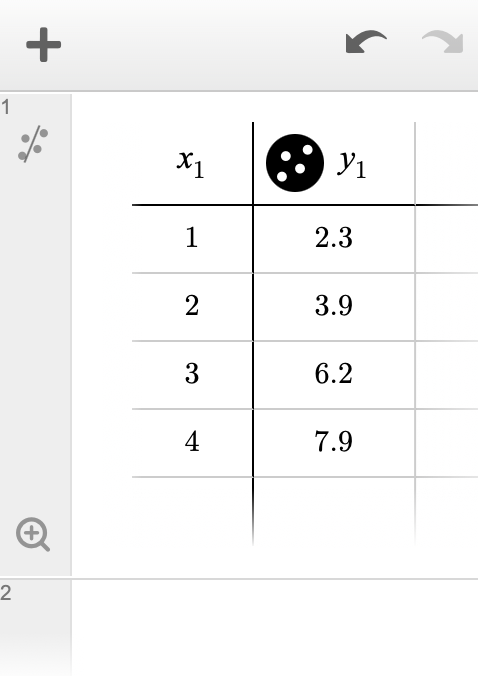
\includegraphics[width=3cm]{desmos1}};


      \node[anchor=north west] at (3.5,0) 
        {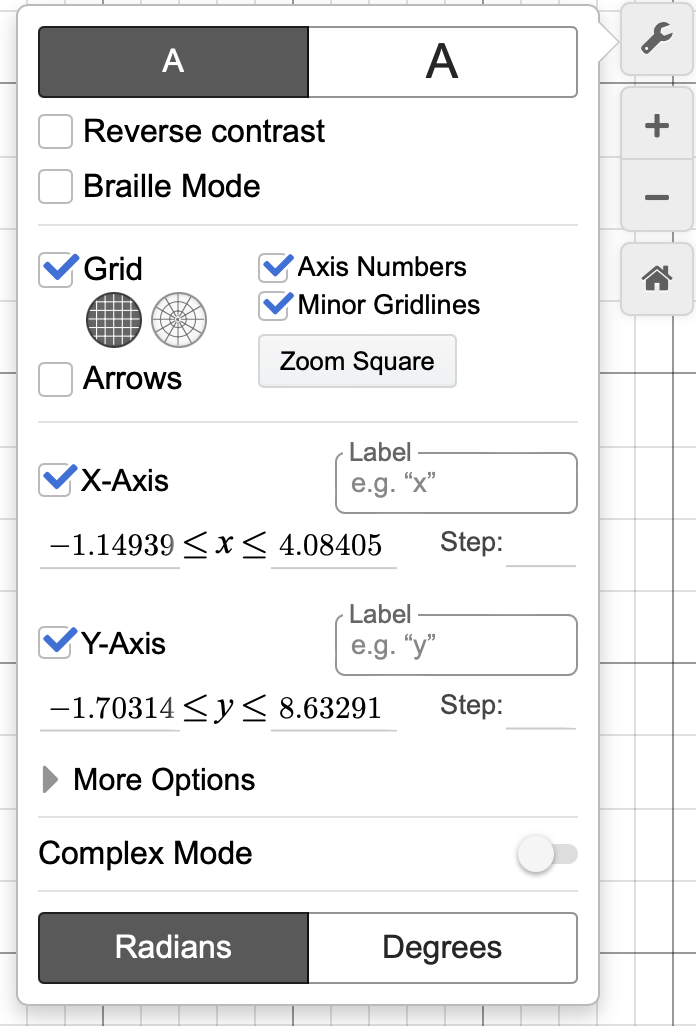
\includegraphics[width=3.5cm]{desmos2}};

          \draw (2,0) 
        node[fill=red!20,rounded corners] (table)
        {\ref{table} Create a table};
      \draw[red] (0.4,-.4) coordinate (a) circle (0.3);
      \draw[<-,red,very thick] (a) +(0.3,0) -- (table.south);

      \node[fill=blue!20,rounded corners] at (2.5,-1.5) (linear) {\ref{linear} Linear Regression};
      \draw[blue] (0.3,-1) coordinate (a) circle (0.3);
      \draw[<-,blue,very thick] (a) +(0.3,0) -- (linear.north);

      \node[fill=green!20,rounded corners] at (2,-2.5) (zoom) {\ref{zoom} Zoom Fit};
      \draw[green, ultra thick] (0.3,-3.5) coordinate (a) circle (0.3);
      \draw[<-,green,very thick] (a) +(0.3,0) -- (zoom.west);

      \node[fill=orange!20,rounded corners] at (4.5,-0.5) (wrench) {\ref{wrench} Axis Labels};
      \draw[orange, ultra thick] (6.9,-.3) coordinate (a) circle (0.3);
      \draw[<-,orange,very thick] (a) +(-0.3,0) -- (wrench.east);

      \draw[->,orange,very thick] (wrench.south) -- (5.2,-2.3);

      \draw[orange, ultra thick, rounded corners] (3.8,-2.3) rectangle ++(2.8,-0.5);
      \draw[orange, ultra thick, rounded corners] (3.8,-3.1) rectangle ++(2.8,-0.5);
    \end{tikzpicture}


\end{multicols}

\pagebreak
\section*{Analysis}

\begin{questions}

  \question
    Try making a best fit line.  How well does this best-fit line represent your data?  Give a reason why a line is not good for this data.
    \vs

  \question
    Instead make of a linear regression, use the drop-down menu on Desmos to change to \textbf{\it ``Quadratic''}.  Write down the formula for the best fit curves

    \begin{multicols}{2}
    

    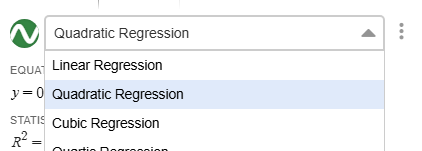
\includegraphics[width=7.5cm]{desmos4}
    
    \vspace{1em}

    Equation:

    \vspace{3em}

    \vspace*{3em}

  \end{multicols}

    \emph{After you've done this, make sure to submit your graph on Schoology}.

  \question
    Comment on the precision of your graph now that there's a curve instead of a linear fit. 
    \vs
      
  \question
    Explain why the shape of the graph makes sense.  
    \vs

  
  \question
    Your graph is not perfect.  What were some aspects that limited the accuracy of our graph and our precision?  What could be done to mitigate these in future experiments?
    \vs
  
  


\end{questions}

\end{document}